\chapter{Конструкторская часть}

В данном разделе будут описаны алгоритмы и структуры данных, выбранные для
решения поставленной задачи, будет разработана структура программно-аппаратного комплекса. 

\section{Структуры данных}

Чтобы формализовать алгоритм синтеза изображения в программе, необходимо определить структуры данных, которые будут в ней использоваться. 
В данной работе приняты следующие соглашения. 
Трёхмерные модели являются полигональными, тогда сцену можно представить в виде массива многоугольников (полигонов). Многоугольник включает в себя следующие данные:

\begin{itemize}
    \item количество вершин;
    \item массив x и y координат вершин;
    \item коэффициенты уравнения поверхности, несущей данный многоугольник заданного в виде $a * x + b * y + c * z = d$;
    \item цвет в цветовой модели RGB~\cite{rgb}.
\end{itemize}

Окна, использующиеся в алгоритме Варнока, имеют прямоугольную форму и хранят следующую информацию:
\begin{itemize}
    \item количество многоугольников, рассматриваемых при изображении данного окна;
    \item массив многоугольников;
    \item координаты x и y левой верхней и правой нижней вершин окна. 
\end{itemize}

Структура камеры содержит:
\begin{itemize}
    \item позицию камеры в объектном пространстве;
    \item координаты точки, в которую направлен обзор камеры;
    \item вектор, направленный вверх;
    \item вектор, направленный вправо.
\end{itemize}

Сцена состоит из объектов в пространстве, камеры и источников света.

\section{Трехмерные преобразования}
Для корректной работы алгоритмов удаления невидимых линий и поверхностей сначала необходимо провести преобразования объектов сцены, заданных в объектном пространстве.

\subsection{Пространство камеры}
Первым преобразованием является переход из системы координат глобального пространоства в пространство камеры (англ. Camera view) \cite{camera}.

\begin{equation}
M_{view} = 
\begin{bmatrix}
    R_x & R_y & R_z & 0 \\
    U_x & U_y & U_z & 0 \\
    D_x & D_y & D_z & 0 \\
    0   &  0  &  0  & 0 \\  
\end{bmatrix}
\times
\begin{bmatrix}
    1 & 0 & 0 & -P_x \\
    0 & 1 & 0 & -P_y \\
    0 & 0 & 1 & -P_z \\
    0 & 0 & 0 & 1    \\  
\end{bmatrix},
\end{equation}
где $U$ -- вектор, задающий камеру и направленный вверх, $R$ -- вектор, задающий камеру и направленный вправо, $D$ -- вектор направления обзора камеры, $P$ -- вектор позиции камеры. $M_{view}$ -- итоговая матрица преобразования произвольного вектора из глобальной системы координат в систему координат камеры.

\subsection{Перспективные преобразования}
Для построения реалистичных изображений необходимо учитывать перспективу трехмерной сцены. Для этого объекты, находящиеся в пространстве камеры, подвергаются перспективному преобразованию.

\begin{equation}
M_{proj} = 
\begin{bmatrix}
    \frac{1}{ar \cdot \tg{\frac{\alpha}{2}}} & 0 & 0 & 0 \\
    0 & \frac{1}{\tg{\frac{\alpha}{2}}} & 0 & 0 \\
    0 & 0 & \frac{-NearZ-FarZ}{NearZ-FarZ} & \frac{2 \cdot FarZ \cdot NearZ}{NearZ-FarZ} \\
    0   &  0  &  1  & 0 \\  
\end{bmatrix},
\end{equation}
где $ar$ -- соотношение сторон изображения (англ. aspect ration), $NearZ$ и $FarZ$ -- координаты Z, ограничивающие область преобразования, $\alpha$ -- угол обзора. $M_{proj}$ -- матрица перспективного преобразования \cite{perspective}. 

Итоговое преобразование вектора из глобальной системы координат, в систему координат, требующуюся для синтеза изображения можно записать в виде:
\begin{equation}
V_{result} = M_{proj} \cdot M_{view} \cdot V_{global},
\end{equation}
где $V_{result}$ -- итоговый вектор, $V_{global}$ -- вектор в глобальной системе координат~\cite{projection}.

\section{Алгоритм работы программно-аппаратного комплекса}

Алгоритм работы программно-аппаратного комплекса представлен в виде диаграммы, оформленной в
соответствии с нотацией IDEF0 и отражающей общую декомпозицию
алгоритма~\cite{idef0}.

\begin{figure}[H]
	\centering
	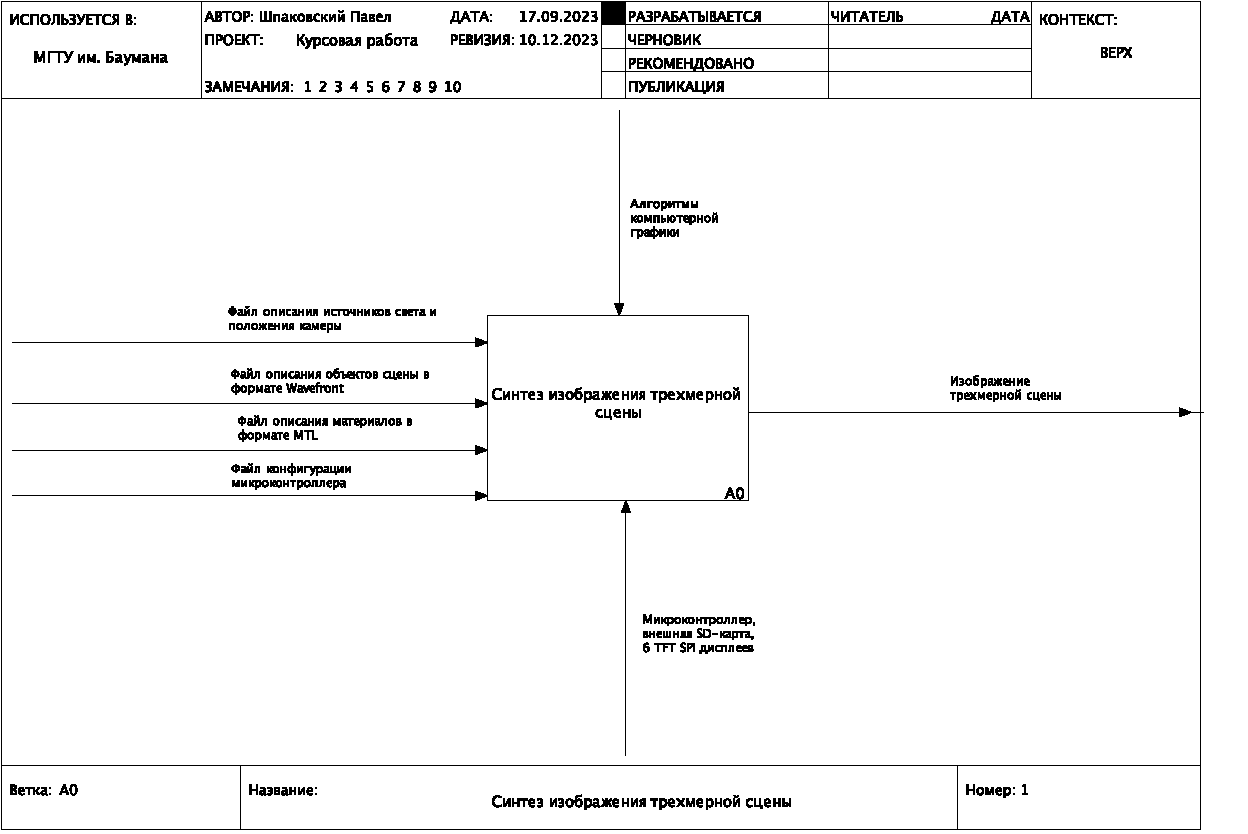
\includegraphics[height=0.45\textheight]{inc/img/01_A0.pdf}
	\caption{Функциональная схема программно-аппаратного комплекса, декомпозиция верхнего уровня}
	\label{fig:a01}
\end{figure}

\begin{figure}[H]
	\centering
	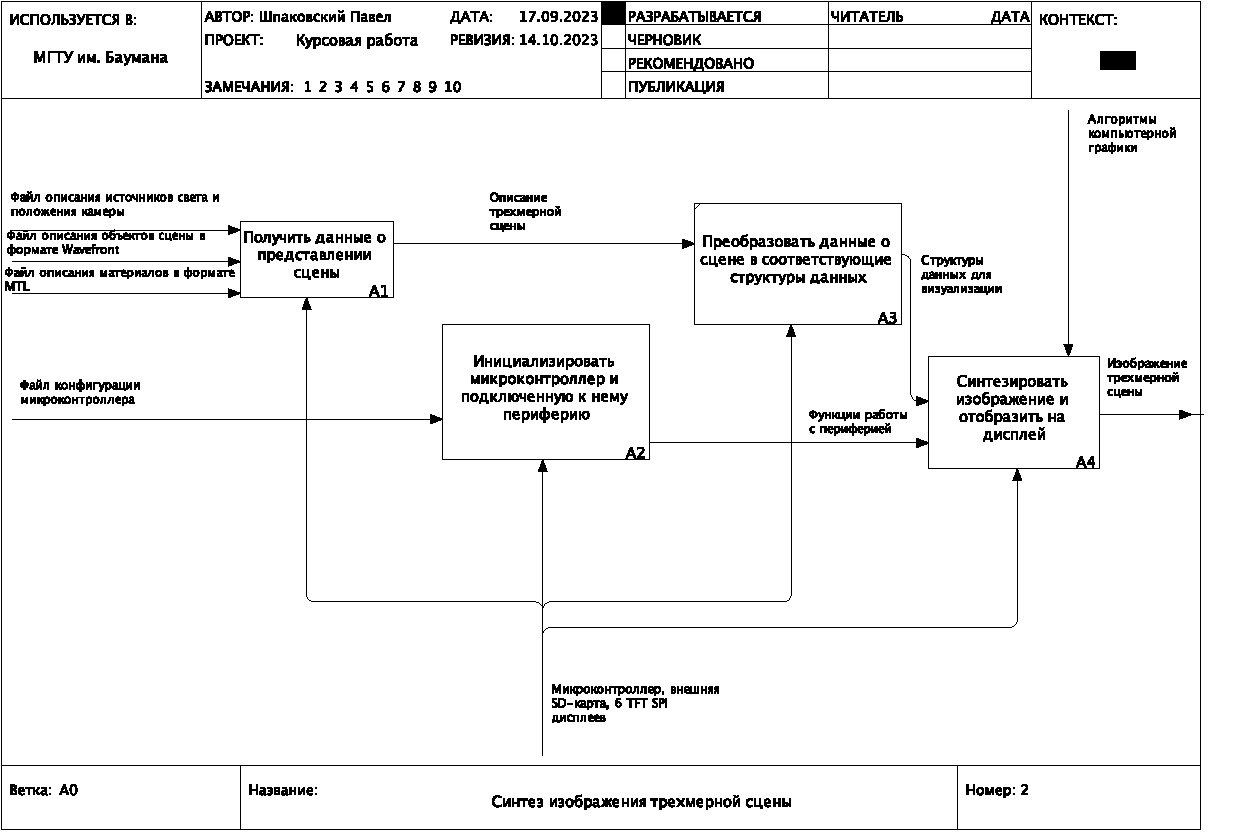
\includegraphics[height=0.45\textheight]{inc/img/02_A0.pdf}
	\caption{Функциональная схема программно-аппаратного комплекса, декомпозиция уровня A0}
	\label{fig:a02}
\end{figure}

\begin{figure}[H]
	\centering
	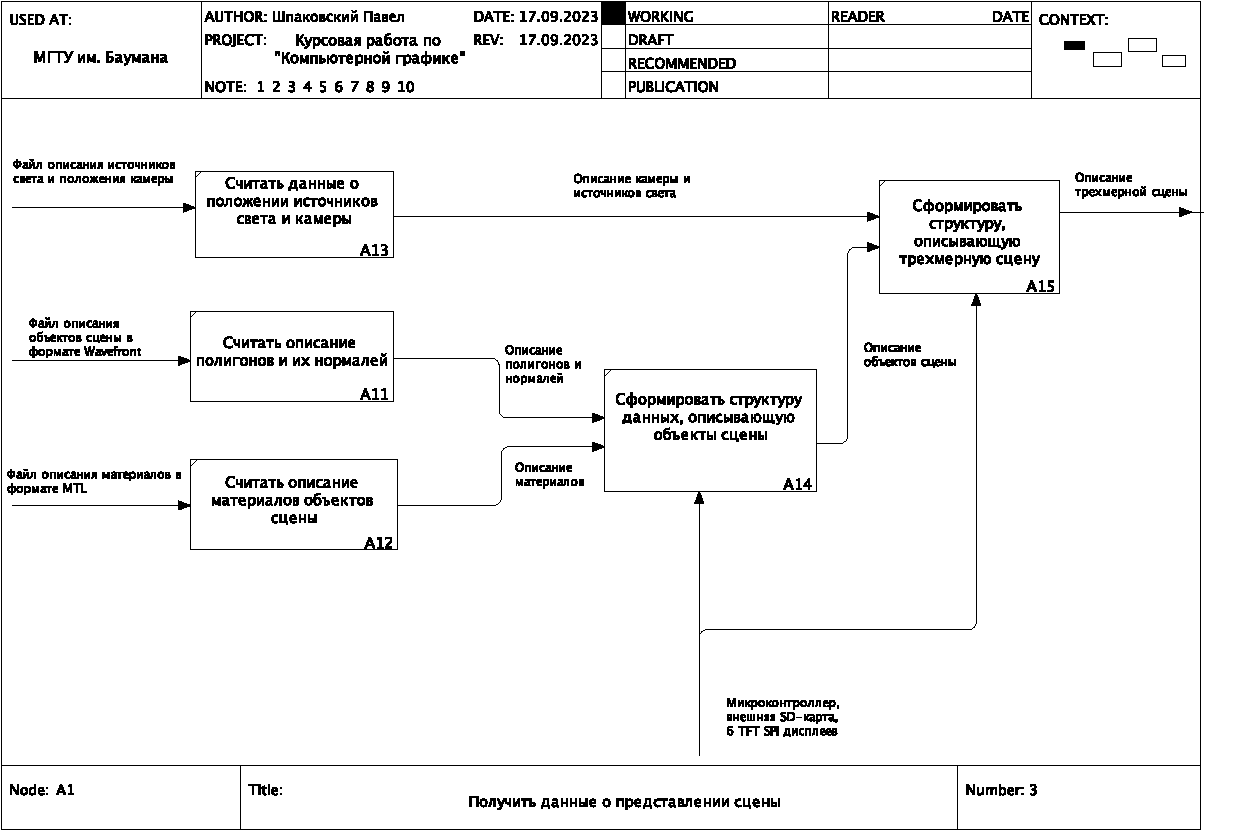
\includegraphics[height=0.45\textheight]{inc/img/03_A1.pdf}
	\caption{Функциональная схема программно-аппаратного комплекса, декомпозиция уровня A1}
	\label{fig:a1}
\end{figure}

\begin{figure}[H]
	\centering
	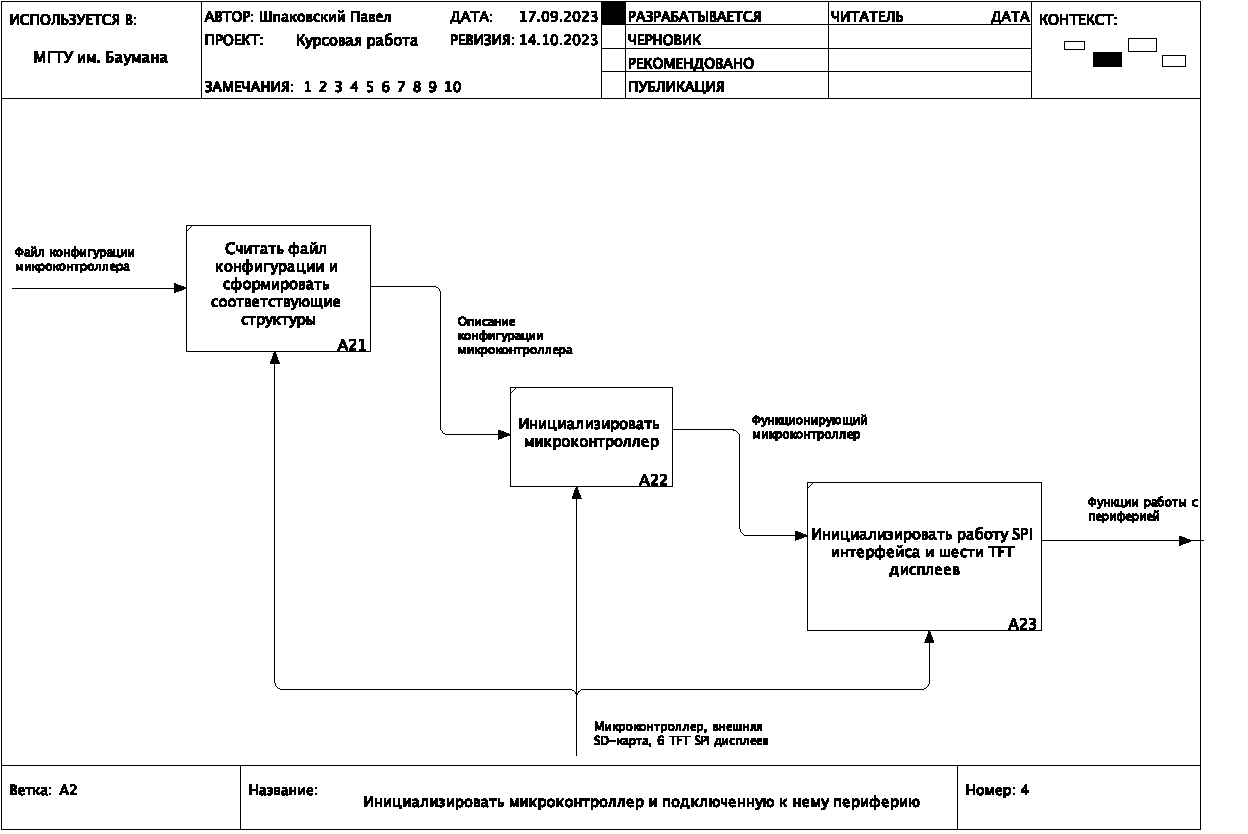
\includegraphics[height=0.45\textheight]{inc/img/04_A2.pdf}
	\caption{Функциональная схема программно-аппаратного комплекса, декомпозиция уровня A2}
	\label{fig:a2}
\end{figure}

\begin{figure}[H]
	\centering
	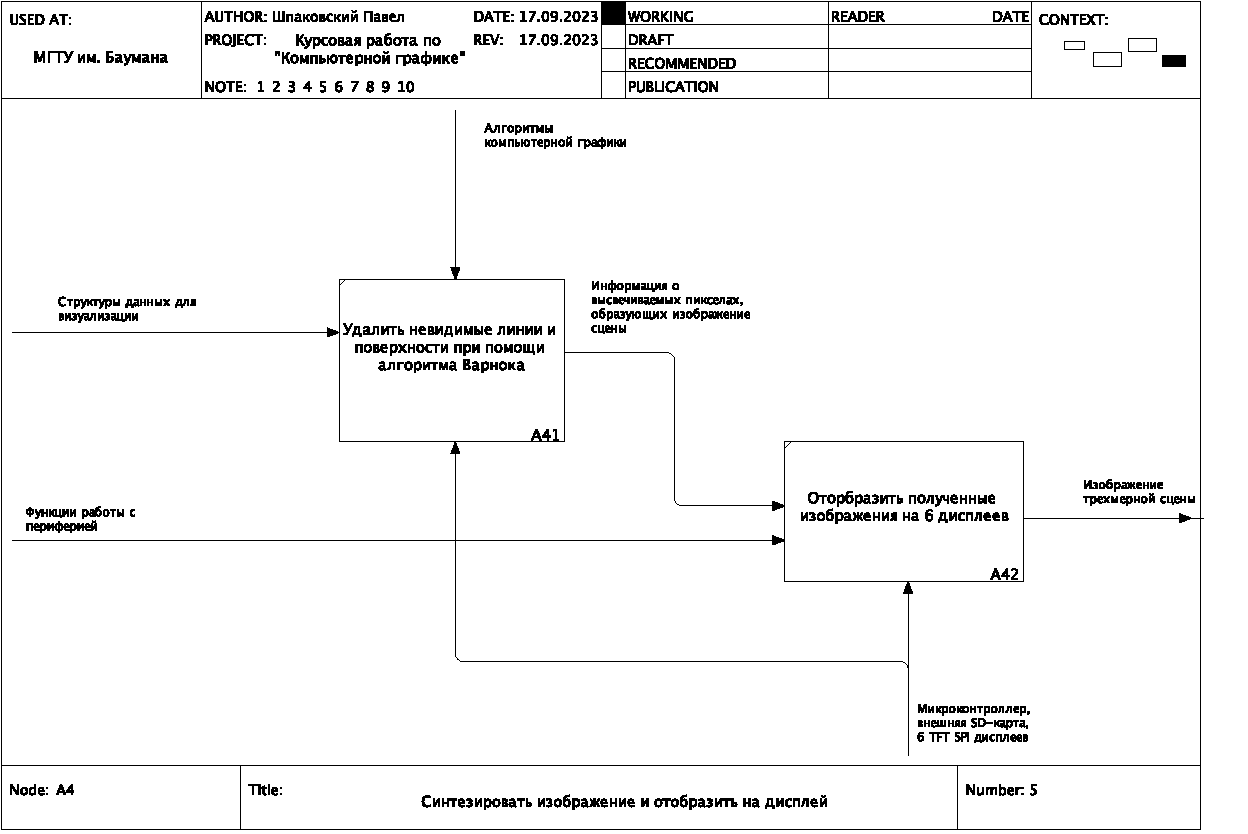
\includegraphics[height=0.45\textheight]{inc/img/05_A4.pdf}
	\caption{Функциональная схема программно-аппаратного комплекса, декомпозиция уровня A4}
	\label{fig:a4}
\end{figure}

\section{Алгоритм Варнока}
Для удаления невидимых линий и поверхностей был выбран алгоритм Варнока, основанный на рекурсивном разбиении окон. 
Под окном в данном алгоритме понимается область изображения на дисплее, которая может содержать визуализируемые объекты сцены. 
Разбиение окон в алгоритме Варнока может быть реализовано как рекурсивно, так и итерационно. 
В данной работе будет рассматриваться итерационная реализация с использованием стека окон, так как она задействует меньший объём памяти, чем рекурсивная.
Схема алгоритма Варнока представлена на рисунке \ref{fig:warnock}.

\begin{figure}[H]
	\centering
	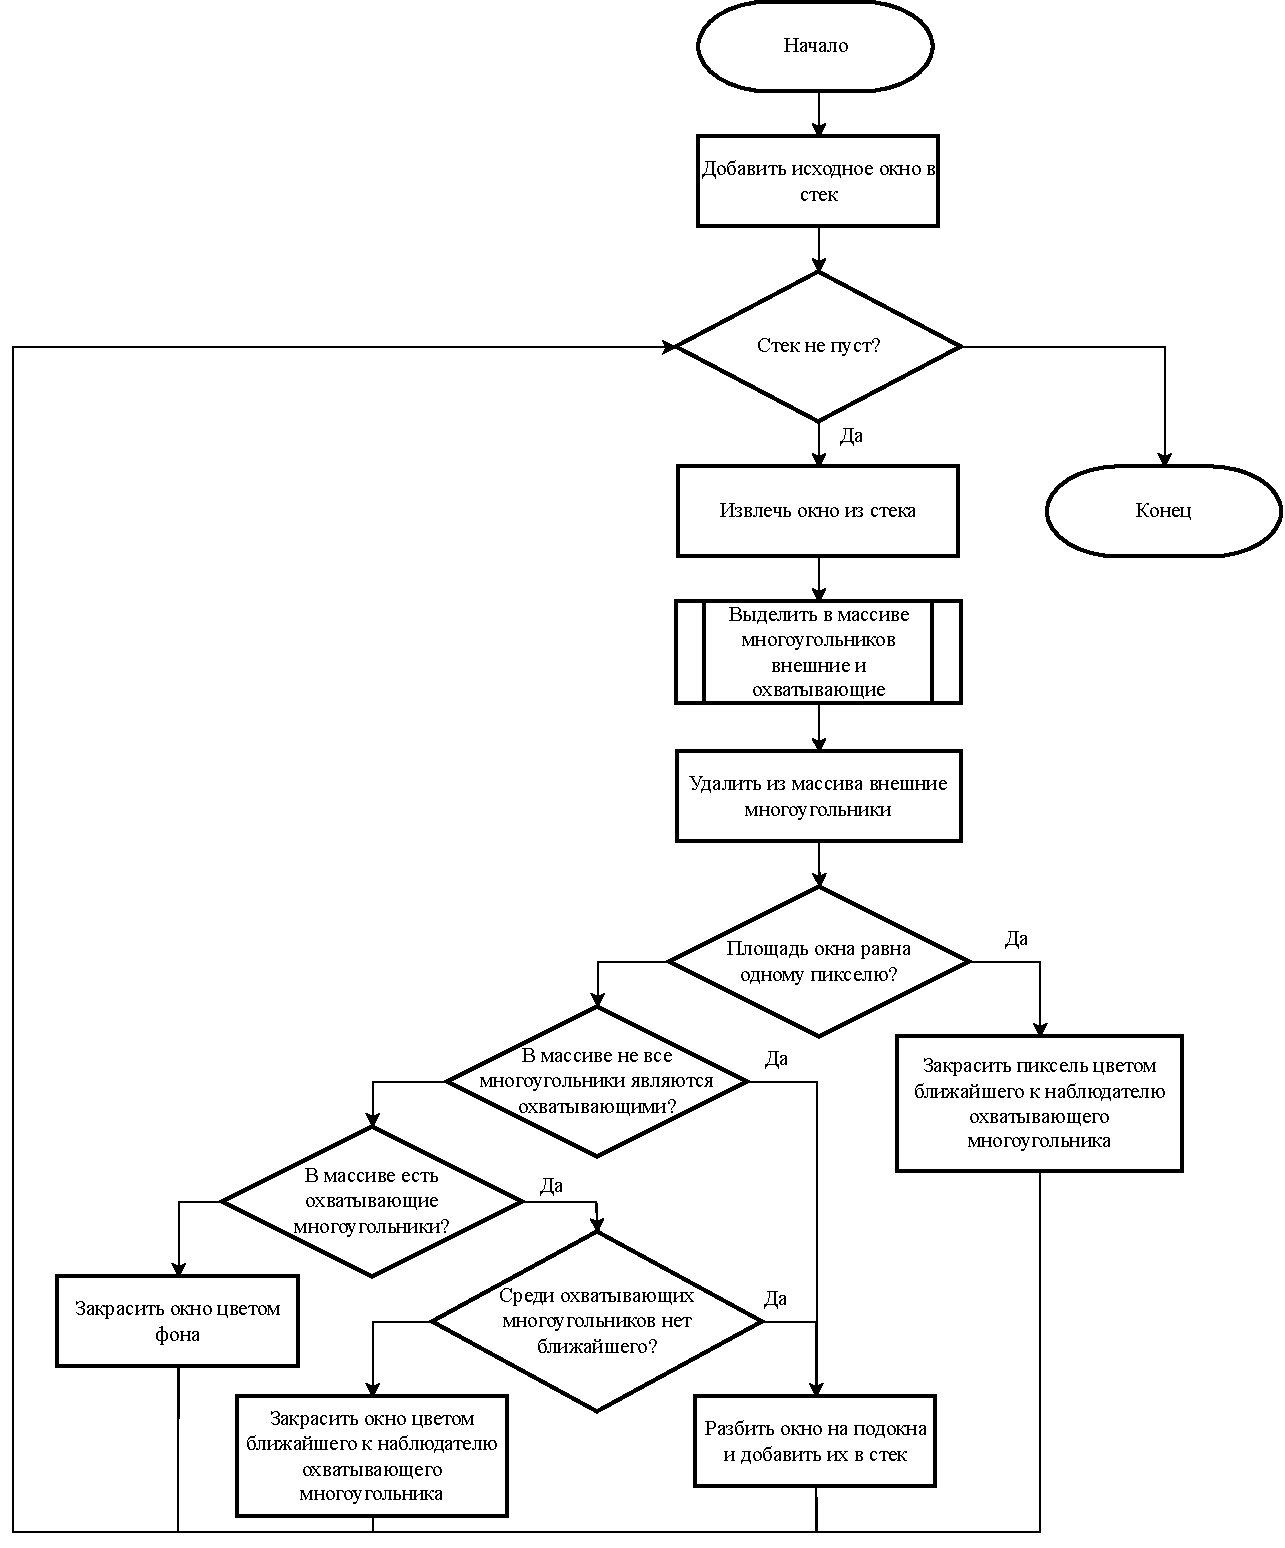
\includegraphics[height=0.75\textheight]{inc/img/warnock.pdf}
	\caption{Схема работы алгоритма Варнока}
	\label{fig:warnock}
\end{figure}

\section{Вывод из конструкторской части}
В данном разделе были описаны алгоритмы и структуры данных, выбранные для решения поставленной задачи и отвечающие требованиям компактности, простоты и быстродействия. 
